\documentclass{article}
\usepackage[utf8]{inputenc}
\usepackage{graphicx}

\title{Combinatorial Analysis of Enigma Machine}
\author{\large Skylar Liang (skylarl), Samie Amriui (samiea) \par}
\date{\normalsize March 10, 2020 \par}

\usepackage{natbib}
\usepackage{lipsum}

\begin{document}

\maketitle

\section{Introduction}
\subsection{The Background of the Enigma Machine}
The Enigma Machine was invented by the German engineer Arthur Scherbius at the end of World War I in 1918 \cite{abny}. It looks like a typewriter that has a light-board with a set of letters above the keyboard, and later on in the history, in order to increase the complexity of the cipher, a plug-board was added to the bottom-front of the machine. During World War II, a Nazi German operator would type the plain text into the Enigma Machine. Each time a letter is pressed, the corresponding letter after the encryption would light up. The operator only needed to copy the letter down and sent it through Morse Code. Decrypting a message is equally as convenient as encrypting since the cipher is one-to-one encryption, under the same machine setting, one only needs to type the encrypted text in and the plain text is revealed through the light-board. \\
\par Originally, the Enigma Machine was created to keep Nazi German communication secret but it was eventually cracked by the Allies during the war which potentially helped significantly shorten the duration of the war and save countless lives by intercepting Nazi German operations and enabled Allies to provide improvisations and counterintelligence operations for them.

\begin{figure}[h!]
\centering 
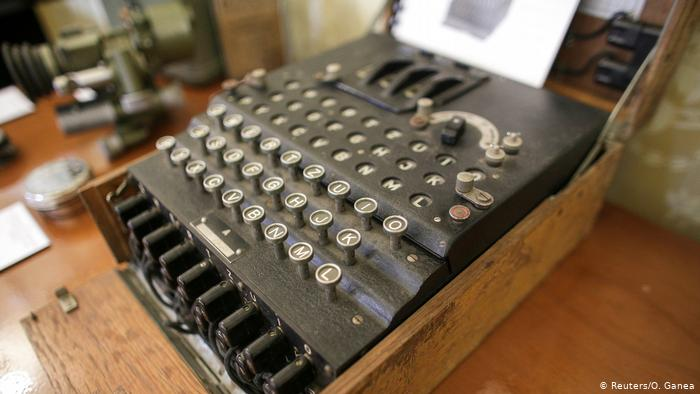
\includegraphics[scale=0.4]{Enigma_Machine.jpg}
\caption{An enigma machine used during WWII}
\label{fig:kuiper-belt}
\end{figure}

\subsection{Interest in the Enigma Machine}
The Enigma Machine feigns the appearance of a regular typewriter but it is a sophisticated cipher machine used to keep radio communications secret. It is an instance of a rotor-based cipher machine that utilizes three rotors. Unlike old-fashioned code, the Enigma Machine will not always light up the same signal for a pressed letter (e.g. two consecutively pressed H would be encrypted as two different letters) due to the rotor movements, which made the Enigma Machine a fascinating and unique method of cryptography of its time.\\
\par The Enigma Machine was an outstanding innovation at that time in history. Nowadays, almost everything on the internet is encrypted in some form and shape. Computers can form so much more sophisticated encrypt ions at the speed of electrons flowing through the computer's processor. As technology progresses, ciphers with more possible combinations will appear and understanding the way to break them will enhance the knowledge we have in cryptography. \\
\par Although the Enigma Machine was ultimately decrypted by Alan Turing, it proved to have immeasurable relevance to today’s development in technology since it introduced the concept of encryption through electrical and mechanical circuits. It brought the idea of secure communication within the scope of modern technologists utilize the advantages and shortcomings that can be learned from the Enigma Machine to create nearly unbreakable encryption that protects our data today.

\section{Combinatorial Theory in the Enigma Machine}

\subsection{Mechanism of Enigma Machine in the Military}

We will talk about how the Enigma Machine operates and the way it encrypts messages. 
\par During WWII, Nazi German operators of the enigma machine would choose three rotors from five possible choices that provide an alphabet order \cite{MLB}. A standard enigma machine can only hold three rotors, and for each rotor, the numbers 1 to 26 are carved on the surface which represents 26 possible starting settings for each rotor. 
\par At the beginning, each time a letter is pressed, the rightmost rotor moves and increases the number by 1. When the rightmost rotor reaches its turnover position, which can be different from its starting point, it will kick the next rotor. Then the middle rotor will move from its starting point which might be different than rotor 1, and once again increases its value by 1 \cite{MLB}. This is the process of turnover, which ensures the number of different encryption one can have while using an Enigma Machine. Thus, the number of possible set up of an Enigma Machine can be very complicated since the rotors are not identical.\\ 
\par Different rotors at different positions provide different numbers of output. For military use, the Enigma Machine also includes an extra set of plug-board that swaps two letters that are manually paired up by the user, as shown in Figure \ref{fig:plug-board}. For a total of 26 letters, there are 10 wires that can be used to connect any two letters together \cite{cac}. Then the encryption of a letter will follow the encryption of its paired up letter instead of itself. 
\par For example, if A is connected with Q, then the output of a letter A would be based on the encryption of Q, and vice versa. The order of the chosen pairs does not matter, it is a two way connection. Once 10 pairs are chosen, there are 6 letters left over that are not connected. For those not connected, their means of encryption will not be changed. 
\par This clearly boosted up the number of possible encryption the Enigma Machine could have. With a Nazi German switching the pairing letters in the plug board every 24 hours, the Allies were in deep trouble trying to decrypt their messages.

\begin{figure}[h!]
\centering 
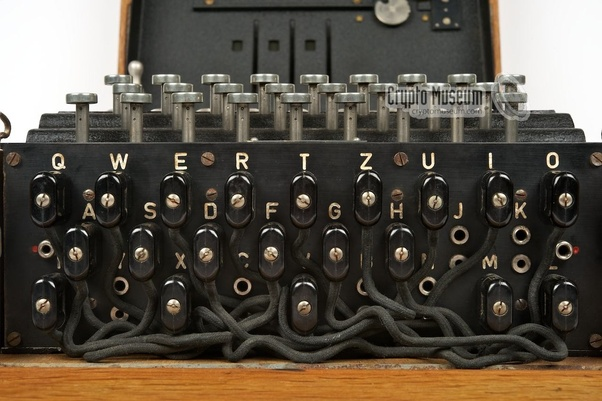
\includegraphics[scale=0.4]{plug board.jpeg}
\caption{The plug board of an Enigma Machine}
\label{fig:plug-board}
\end{figure}

\subsubsection{Example of the Encryption and Decryption Process} 
\textit{Set up instruction:} 215 AAA FRA "ABIRUXKP" \\
\textit{Plain text:} ANBULMEGRAZGOESTINGSTRENGGEHEIMEMELDUNG \\
\textit{Explanation of the set up instructions: }
\par 215 - rotor order, means left wheel number 2, middle wheel number 1 and right wheel number 5. 
\par AAA is the corresponding ring setting.
\par FRA is the corresponding starting position.
\par AB IR UX KP Plugboard connections. \\
\textit{Encrypted text:} PCDAONONEBCJBOGLYMEEYGSHRYUBUJHMJOQZLEX
    \begin{table}[hbt!]
    \caption{Turnover positions of each available rotor in the Enigma Machine}
    \centering 
    \begin{tabular}{c|c|c}
    \hline\hline 
    Rotor & Turnover Position(s) & BP mnemonic  \\
    \hline 
    I & R & Royal    \\
    II & F & Flags   \\
    III & W & Wave  \\
    IV & K & Kings \\
    V & A & Above  \\
    VI, VII, and VIII & A and N & - 
    \end{tabular}
    \end{table}

\subsection{The Number of Possible Encryption with the Enigma Machine}
First of all, for each section, we calculated the possible number of combination separately. \\
First, we calculate all the possibilities of the plug-board.
\par Since there are $10$ wires connecting $20$ letter, there are 6 letters being left out. So we treat those 6 wires as repeats. The wires of each pair is different than other pairs, so we want to choose 10 pairs. And in each pair, there are $2$ ways of arranging the letters, so total of ten 2s: $P(26; 6, 10, 2, 2, ... , 2) = \frac{26!}{6!10!2!^{10}}$ ways \\
Second, we calculate possible ways to pick rotors from the box, assuming all the rotors are identical, and the total number of rotors is 5.
\par Picking 3 rotors from a total of 5 rotors: ${5}\choose{3}$ ways \\
Third, we calculate the number of possible ways to pick the starting position of all three rotors. 
\par Picking starting positions: $26 * 26 * 26 = 26^{3}$ ways by m.p.
\par We use multiplication principle here since the steps performed in this combinatorial situation are connected, therefore the number of possible settings by multiplication principle is as follows \cite{cac}: \\
        $\frac{26!}{6!10!2!^{10}}$ $\cdot$ ${5}\choose{3}$ $\cdot$ $26^{3}$

\section{Conclusion}
By calculating the number of possible ways of encryption of an Enigma Machine, we know that it was not possible for the Allies to break it without an algorithmic solution. With the number of combinations used for a military standard Enigma Machine totaling in the hundreds of billions, it was no wonder that the Enigma Machine was originally thought to be unbreakable. 

\bibliographystyle{plain}
\bibliography{references}
\end{document}
